\begin{figure}[!tp]
	\centering
	\begin{minipage}[!t]{\textwidth}
		\centering
		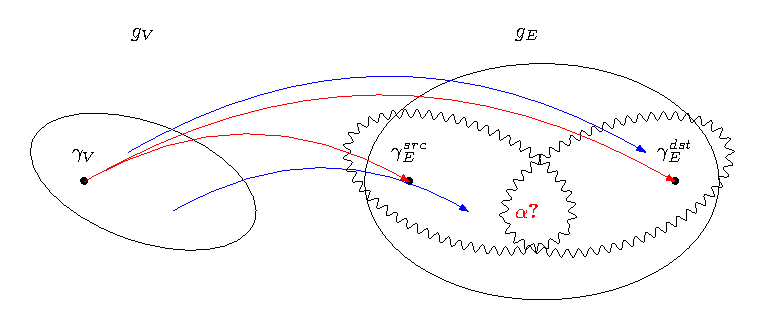
\includegraphics[width=\textwidth]{fig/06nesting/01_preliminar_question.pdf}
		\subcaption{Comparing the vertex summarization pattern and the path summarization patterns. We suppose that edge grouping references ($\gamma_E^{src}$ and $\gamma_E^{dst}$) correspond to the same vertex appearing as a vertex grouping reference ($\gamma_V$) Such correspondence is directly marked my the user itself providing the query by drawing morphisms (correspondences) between the vertex and the path summarization patterns (red edges). The intersections between the two patterns may be directly outlined by the user itself that provides the query (blue edges, representing other morphisms).}
		\label{fig:patcomparison}
	\end{minipage} \begin{minipage}[!t]{0.45\textwidth}
		\centering
		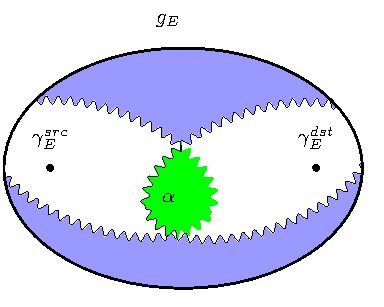
\includegraphics[width=1\textwidth]{fig/06nesting/02_edge_analysis.pdf}
		\subcaption{Path summarization pattern sharing an $\alpha$ area of common patterns shared between the patterns, which are necessairly not the edge grouping references by definition.}
		\label{fig:edgewithIntersectionNonSRC}
	\end{minipage}\quad \begin{minipage}[!t]{0.45\textwidth}
		\centering
		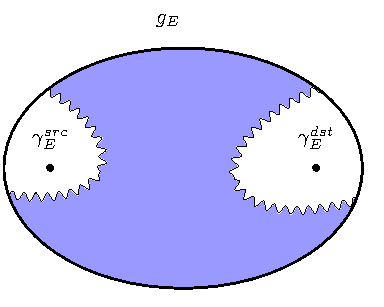
\includegraphics[width=1\textwidth]{fig/06nesting/03_edge_analysis.pdf}
		\subcaption{Path summarization pattern not sharing a common $\alpha$ area, although $\gamma_E^{src}$ and $\gamma_E^{dst}$ must always be present in $g_E$ by hypothesis. This constraint guarantees that the newly created edge will be associated to a nested vertex originating from the vertex summarization pattern.}
		\label{fig:edgeWithNoIntersection}
	\end{minipage}
	\caption{Vertex (V) and Path (E) summarization patterns for the query expressed in Example \vref{ex:nestingbib}. Vertex and edge grouping references are marked by a light blue circled node. As we can see, the vertex grouping reference depicts the same property expressed by edge grouping references.}
	\label{fig:patternAnalysis}
\end{figure}
\section{Class of optimizable graph nesting queries}\label{sec:optimizableClass}
Before defining the general graph nesting operator and its THoSP algorithm, this seection detects the broader class of vertex and path summarization patterns optimizable as discussed in the chapter's introduction. The generation of the collections is only relevant with respect to actual data that is going to be nested and, in our case, we can only nest a subgraph of the graph resulting from the graph visiting process: consequently, within each pattern we must remark which elements are going to be nested at the final result. Instead of traversing a graph, generating the collections to be nested within the graph and check which one of them can be actually nested, we can directly create the nested graph while visiting the property graph.

First, we must provide a formal characterization of the grouping reference: we want to elect a subgraph $\gamma_p$ for each graph pattern $g_p$ such that each graph generated by the morphisms\footnote{See Definition \vref{sec:graphamatch} for a back reference.} $m_{g_p}(\nested)$ expose unique elements referring to $\gamma_p$. These grouping references elect the subcomponents identifying an entity over which the aggregation will be performed during the graph matching process. Hereby, we can provide the following formal definition for grouping references:
\begin{definition}[Grouping reference]
Given a graph pattern $g_p$ generating a set of morphisms $m_{g_p}(\nested)$ over a nested graph $\nested$, a \textbf{grouping reference} $\gamma_p$ is a subpattern $\gamma_p\subseteq g_p$ restricting the possible morphisms generated by $m_{g_p}(\nested)$ to the $f_i$ such that $|f_i(o)|=1$ for each object $o\in O_{\gamma_p}$ and that another morphism $f_j\neq f_i$ is such that $f_i(O_{\gamma_p})\neq f_j(O_{\gamma_p})$.
\end{definition}

If we reduce the grouping references to one single vertex for vertex summarization patterns, and to two (distinct) vertices for path summarization patterns, we may reduce the computational complexity of aggregating the grouping reference. As already sketched by the introduction, the class of the desired nesting algorithms create new nested edges only over vertices that will be  matched as grouping references and then nested. Moreover, we can choose to mark with a specific $\xi$ value (e.g. \mstr{toNest}) each pattern vertex and pattern edge to explicitely state which elements have to be nested in the final result; this implies that \textsc{User Defined Functions} are directly required to create the matched vertices and edges because they can be directly represented within the graph patterns.

Figure \vref{fig:patternAnalysis} provides an example on how  graph nesting queries based on grouping references can be optimized for both vertex ($g_V$) and path ($g_E$) summarization queries; given that the users are going to provide both the vertex and the path summarization queries, such users must directly draw the correspondences between vertex and edge pattern queries, so that the correspondences can be promptly be identified by the query plan which can better optimize the whole query execution (\subref{fig:patcomparison}). After doing so, we can start to perform the general graph visiting algorithm for graph nesting (Algorithm \ref{alg:general}) by detecting which regions of both patterns are shared together in $\alpha=g_V\cap g_E$ (Figure \ref{fig:edgewithIntersectionNonSRC}). Given that path summarization patterns' grouping references have distinct source and destination vertices  by definition, source and destination vertices may not be represented in $\alpha$ (line \ref{obtainAlpha}). Consequently, we can first perform pattern matching over the input graph over $\alpha$, thus allowing a partial instantiation of the $g_V$ and $g_E$ patterns, and then iteratively extend the nesting information after each visit of $\alpha$ and  its own refinements. In particular, we can perform the algorithm  as follows:
\begin{algorithm}[!t]
	\caption{Grouping Reference Optimizable Queries (GROQ)}\label{alg:general}
	\begin{adjustbox}{max width=\textwidth}
		\begin{minipage}{1.2\linewidth}
			\begin{algorithmic}[1]
				\State {\textbf{new} $\nested' := (\ngraph_{c+1}, O,\ell,\xi,\phi)$}
				\State
				\Procedure{GROQ}{$(g_V,\gamma_V),({g_E},\gamma_E^{src},\gamma_E^{dst}),m;\;\nested$}:\Comment{$\nested=(\ngraph_c,O,\ell,\xi,\phi)$}
				\State {$\alpha:=g_V\cap {g_E}\backslash(\gamma_V\cup\gamma_E)$;}\label{obtainAlpha}
				\State {lV $:=$ [];}
				\If{$\alpha\neq\emptyset$}
					\For {\textbf{each graph} $g^i$ generated from $m_\alpha(\nested)$ }\label{eachAlpha}
						\State {lV $:=\{f_i\in m_{g_V;\gamma_V}(\nested)|f_i(\alpha)=g^i\}$}
						\State {GROQ$\alpha$}{($(g_V,\gamma_V),({g_E},\gamma_E^{src},\gamma_E^{dst}),m;\;\textup{lV},\nested$)}
					\EndFor
				\Else
					\State {lV $:=m_{g_V;\gamma_V}(\nested)$}\label{complete}
					\State {GROQ$\alpha$}{($(g_V,\gamma_V),({g_E},\gamma_E^{src},\gamma_E^{dst}),m;\;\textup{lV},\nested$)}
				\EndIf
				
				\EndProcedure
				\State
				\Procedure{GROQ$\alpha$}{$(g_V,\gamma_V),({g_E},\gamma_E^{src},\gamma_E^{dst}),m;\;\textup{lV},\nested$}
				\For {\textbf{each morphism} $f_i\in\; $lV}
				\State {$\{{i}_c\}:=f_i(\gamma_V)$}\label{vertexReferencePatt}
				\State {$\ell(i_{c+1}):=\ell(i_c);\; \xi(i_{c+1}):=\xi(i_c);\; \phi(i_{c+1})=\phi(i_{c+1})|_{\dom(\phi(i_{c+1}))\backslash\{\ONTA,\RELA\}}$}\label{vertexLVPreserve}
				\State {$\phi(\ngraph_{c+1},\ONTA):=\phi(\ngraph_{c+1},\ONTA)\cup \{{i}_{c+1}\}$}\label{vertexGeneration}
				\State {$\phi({i}_{c+1},\ONTA):=\phi({i}_{c+1},\ONTA)\cup\Set{f_i(o)|o\in O_{g_V},\mstr{toNest}\in\xi(o)\wedge o\in \phi(o_{g_V},\ONTA)}$}\label{vertexContent1}
				\State {$\phi({i}_{c+1},\RELA):=\phi({i}_{c+1},\RELA)\cup\Set{f_i(o)|o\in O_{g_V},\mstr{toNest}\in\xi(o)\wedge o\in \phi(o_{g_V},\RELA)}$}\label{vertexContent2}
				\EndFor
				\For {\textbf{each morphism} $f_i,f_j\in\; $lV}
				\State{lE $:=\{f_k\in m_{{g_E};\gamma_E^{src},\gamma_E^{dst}}(\nested)|f_i(\gamma_V)=f_k(\gamma_E^{src}),f_j(\gamma_V)=f_k(\gamma_E^{dst})\}$}\label{fulTraverse}
				\For {\textbf{each morphism} $f_k\in\; $lE}
				\State {$\{s_c\}:=f_i(\gamma_E^{src})$;\qquad $\{d_c\}:=f_i(\gamma_E^{dst})$}\label{pathReferencePatt1}
				\State {$\omega:=dt(s,d)$}\label{pathReferencePatt2}
				\State {$\ell(\omega_{c+1}):=\ell(s_c)\cup\ell(d_c);\; \xi(i_{c+1}):=\xi(i_c)\cup\ell(d_c)$}\label{fromNewElements}
				\State {$\phi(\omega_{c+1},\RELA):=\phi(\omega_{c+1},\RELA)\cup f_k(\gamma_V)$}\label{edgeGeneration}
				\State {$\phi(\omega_{c+1},\SRC):=\{s_{c+1}\}$;\qquad $\phi(\omega_{c+1},\DST):=\{d_{c+1}\}$}
				\State {$\phi(\omega_{c+1},\ONTA):=\phi(\omega_{c+1},\ONTA)\cup\Set{f_k(o)|o\in O_{g_E},\mstr{toNest}\in\xi(o)\wedge o\in \phi(o_{g_E},\ONTA)}$}
				\State {$\phi(\omega_{c+1},\RELA):=\phi(\omega_{c+1},\RELA)\cup\Set{f_k(o)|o\in O_{g_E},\mstr{toNest}\in\xi(o)\wedge o\in \phi(o_{g_E},\RELA)}$}
				\EndFor
				\EndFor
				\EndProcedure
				
			\end{algorithmic}
	\end{minipage}
	\end{adjustbox}
\end{algorithm}

\begin{itemize}
\item Given a graphs extraction language $m$ (not necessarily) supporting grouping references, we extract all the subgraphs $g^i$ of $\nested$ generated by morphisms $m_\alpha(\nested)$, when $\alpha$ is not empty (line \ref{eachAlpha}). If $\alpha$ is otherwise an empty pattern, we must necessarily perform a complete visit of the vertex patterns $g_V$, and perform complete instantiations of such patterns (line \ref{complete}). 
\item Given that the nested graph representation relies on the GSM model, we can iteratively construct the nested graph without knowing the complete information by relying on the ids of the expected elements, and we can provide the greatest subgraph of $g$ matching $\alpha$  after visiting  each possible $\alpha$ matching result, represented as a morphism $f_i$. For this reason, the GROQ$\alpha$ subroutine may be called in both cases.

\item After providing a partial instantiation of the vertex summarization patterns via $\alpha$, we find a vertex $i_c$ matching the grouping reference $\gamma_V$ to which we are going to nest the remaining objects: from $i_c$ we generate a newly derived vertex $i_{c+1}$ %start to generate a new nested vertex: this new vertex $i_{c+1}$ descends from the object $i_c$ matched by the grouping reference $\gamma_V$ 
 (line \ref{vertexReferencePatt}) preserving all the labels, expressions and containments of $i_c$ (except from \RELA and \ONTA -- line \ref{vertexLVPreserve}). In particular, the nesting content of $i_{c+1}$ derives from the partial instantiation of the morphism $f_i$, by choosing the vertices and edges in $\nested$ which corresponds to vertex summarization objects marked with \mstr{toNest} (lines \ref{vertexContent1} and \ref{vertexContent2}).

\item At this point we can use the same semi-instantiated morphisms in \texttt{lV} from $\alpha$ to partially instantiate the path summarization pattern, that  is now going to be fully traversed (line \ref{fulTraverse}). For each of these $f_i$ instantiations, new edges are going to be generated, inheriting the labels, values and containments (except from \RELA and \ONTA) from the matched edges grouping references, $s_c$ and $d_c$. In particular, we can directly create associate to such edge the soruces and the targets represented by nested vertices, which will respectively be $s_{c+1}$ and $d_{c+1}$.

\item The procedure is iterated until the whole graph is not visited via subsequent morphisms, and hence all the matched elements are associated from the objects $i_{c+1}$ (either vertices or edges) generated from the ones matched by the grouping reference $i_c$.
\end{itemize}

As we can see from the algorithm, the advantage of this approach is that the graph $g^i$ and the instantiated morphisms (as a consequence of the graph matching phase) are promptly used to define the nested information (e.g., lines \ref{vertexGeneration}-\ref{vertexContent2}). It is evident that the aforementioned algorithm provides the best performances when $\gamma_E^{src}$ and $\gamma_E^{dst}$ are separated by  one edge distance in $\alpha$   and both $g_V$ and $g_E$ create graph collections that are partitions of $\nested$. On the other hand, this class of algorithms was already discussed in literature and, consequently, an approach describing how to optimize such  scenarios can be already found in literature \cite{JunghannsPR17}. Nevertheless, this chapter focuses on another types of algorithms, which are the ones where $\alpha$ contains two edges and one vertex; this class of problems, to the best of our knowledge, has not been discussed yet in current literature with respect to their optimizations. %Therefore, the next paragraph is going to introduce one specific algorithm for $\alpha\neq\emptyset$, where in particular $\alpha$ is formed by one single vertex.
 Please note that, when $\alpha=\emptyset$, the computational complexity of the algorithm may easily become quadratic ($|\phi(\ngraph,\ONTA)|+|\phi(\ngraph,\ONTA)|^2$).
